%% 由 build/emit_tex.py 生成（生成物，勿手改）；定制请放 user_style.tex / user_meta.yaml
\chapter{第 5 章 ·
留数理论及其应用}\label{ux7b2c-5-ux7ae0-ux7559ux6570ux7406ux8bbaux53caux5176ux5e94ux7528}

\section{5.1 留数}\label{ux7559ux6570}

\begin{quote}
\textbf{本节目标}：理解留数的定义与几何意义，掌握留数定理及其证明，熟练运用极点的留数计算公式以及``商函数''留数公式，并了解无穷远点留数的概念与``全体奇点留数之和为零''的定理。
\textbf{重点}：留数的定义、留数定理、极点留数的计算（\(m\) 阶极点公式与
\(P(z)/Q(z)\) 公式）。
\textbf{难点}：无穷远点的留数概念，以及用洛朗展开求 \(a_{-1}\) 的技巧。
\end{quote}

\subsection{5.1.1 留数的定义}\label{ux7559ux6570ux7684ux5b9aux4e49}

设 \(z_0\) 是 \(f(z)\)
的\textbf{孤立奇点}。那么，对于解析圆环(去心邻域)内包含 \(z_0\)
的正向简单闭曲线 \(C\)，积分

\[
\oint_C f(\zeta)\,\mathrm d\zeta
\]

只与 \(f(z)\) 和 \(z_0\) 有关，而与 \(C\)
的选择无关；但该积分值不一定为零。

\(f(z)\) 在 \(z_0\) 的去心邻域内可展开成\textbf{洛朗级数}：

\[
f(z)=\sum_{n=-\infty}^{\infty}a_n\,(z-z_0)^{n},
\]

其中

\[
a_n=\frac{1}{2\pi\mathrm i}\oint_C\frac{f(\zeta)}{(\zeta-z_0)^{n+1}}\,\mathrm d\zeta,\qquad n=0,\pm1,\pm2,\ldots
\]

特别地，当 \(n=-1\) 时，

\[
a_{-1}=\frac{1}{2\pi\mathrm i}\oint_C f(\zeta)\,\mathrm d\zeta .
\]

\textbf{定义 5.1（留数）} 把 \(f(z)\) 在 \(z_0\) 处的洛朗级数中
\((z-z_0)^{-1}\) 项的系数 \(a_{-1}\) 称为 \(f(z)\) 在孤立奇点 \(z_0\)
处的\textbf{留数}，记作

\[
\operatorname{Res}\bigl[f(z),z_0\bigr]=a_{-1},
\]

即

\[
\operatorname{Res}\bigl[f(z),z_0\bigr]
=\frac{1}{2\pi\mathrm i}\oint_C f(z)\,\mathrm dz .
\]

\textbf{例 5.1} 求下列积分的值，其中 \(C\) 为包含 \(z=0\)
的简单正向闭曲线：

\[
(1)\ \oint_C z^{-3}\cos z\,\mathrm dz;\qquad
(2)\ \oint_C \mathrm e^{\frac{1}{z^{2}}}\,\mathrm dz .
\]

\textbf{解} （1）令 \(f(z)=z^{-3}\cos z\)，则 \(z=0\) 为 \(f(z)\)
的孤立奇点。由

\[
\cos z=1-\frac{z^{2}}{2!}+\frac{z^{4}}{4!}-\frac{z^{6}}{6!}+\cdots,\qquad |z|<\infty,
\]

得

\[
f(z)=\frac{1}{z^{3}}-\frac{1}{2}\cdot\frac{1}{z}+\frac{z}{4!}-\frac{z^{3}}{6!}+\cdots,\qquad 0<|z|<\infty .
\]

所以 \(\operatorname{Res}\bigl[f(z),0\bigr]=-\dfrac12\)，从而

\[
\oint_C z^{-3}\cos z\,\mathrm dz=-\pi\mathrm i .
\]

（2）令 \(f(z)=\mathrm e^{1/z^{2}}\)，则 \(z=0\) 为 \(f(z)\)
的孤立奇点。由

\[
\mathrm e^{\zeta}=1+\frac{\zeta}{1!}+\frac{\zeta^{2}}{2!}+\cdots+\frac{\zeta^{n}}{n!}+\cdots,\qquad |\zeta|<\infty,
\]

以 \(\zeta=\dfrac{1}{z^{2}}\) 代入，得

\[
f(z)=1+\frac{1}{1!}\cdot\frac{1}{z^{2}}+\frac{1}{2!}\cdot\frac{1}{z^{4}}+\cdots+\frac{1}{n!}\cdot\frac{1}{z^{2n}}+\cdots,\qquad 0<|z|<\infty .
\]

此展开式中不含 \((z-0)^{-1}\) 项，所以
\(\operatorname{Res}\bigl[f(z),0\bigr]=0\)，于是

\[
\oint_C \mathrm e^{1/z^{2}}\,\mathrm dz=0 .
\]

\subsection{5.1.2 留数定理}\label{ux7559ux6570ux5b9aux7406}

\textbf{定理 5.1（留数定理）} 设函数 \(f(z)\) 在区域 \(D\)
内除有有限个孤立奇点 \(z_1,z_2,\ldots,z_n\) 外处处解析，\(C\) 是 \(D\)
内包围这些奇点的一条正向简单闭曲线，那么

\[
\oint_C f(z)\,\mathrm dz
=2\pi\mathrm i\sum_{k=1}^{n}\operatorname{Res}\bigl[f(z),z_k\bigr].
\]

\begin{figure}
\centering
\pandocbounded{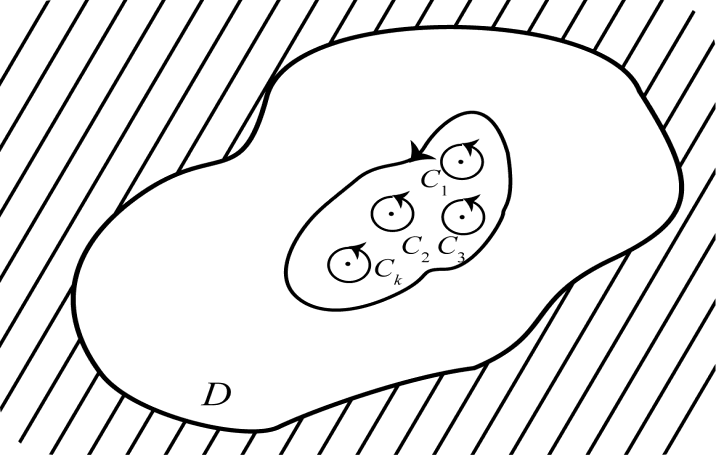
\includegraphics[keepaspectratio,alt={图5.1 留数定理：包围奇点的复合闭路}]{figures/05-留数理论及其应用/fig-p06-5116eeae.png}}
\caption{图5.1 留数定理：包围奇点的复合闭路}
\end{figure}

\textbf{证明要点} 以 \(z_k\) 为圆心，作完全含在 \(C\)
内且互不相交的正向小圆

\[
C_k:\ |z-z_k|=\delta_k,\qquad (k=1,2,\ldots,n).
\]

由复合闭路上的柯西积分定理，有

\[
\oint_C f(z)\,\mathrm dz
=\oint_{C_1} f(z)\,\mathrm dz
+\oint_{C_2} f(z)\,\mathrm dz
+\cdots+\oint_{C_n} f(z)\,\mathrm dz .
\]

但由留数的定义，

\[
\oint_{C_k} f(z)\,\mathrm dz=2\pi\mathrm i\operatorname{Res}\bigl[f(z),z_k\bigr],\qquad k=1,2,\ldots,n,
\]

故

\[
\oint_C f(z)\,\mathrm dz
=2\pi\mathrm i\sum_{k=1}^{n}\operatorname{Res}\bigl[f(z),z_k\bigr].
\]

\subsection{5.1.3
留数的计算方法}\label{ux7559ux6570ux7684ux8ba1ux7b97ux65b9ux6cd5}

\subsubsection{\texorpdfstring{(1) \(m\)
阶极点的留数公式}{(1) m 阶极点的留数公式}}\label{m-ux9636ux6781ux70b9ux7684ux7559ux6570ux516cux5f0f}

\textbf{公式 5.1} 如果 \(z_0\) 为 \(f(z)\) 的 \(m\) 阶极点，那么

\[
\operatorname{Res}\bigl[f(z),z_0\bigr]
=\frac{1}{(m-1)!}\lim_{z\to z_0}\frac{\mathrm d^{\,m-1}}{\mathrm d z^{\,m-1}}
\Bigl\{(z-z_0)^{m}\,f(z)\Bigr\}.
\]

\textbf{证明要点} 因为 \(z_0\) 是 \(f(z)\) 的 \(m\) 阶极点，故在 \(z_0\)
的邻域中有

\[
f(z)=\frac{g(z)}{(z-z_0)^{m}},
\]

其中 \(g(z)\) 在 \(z_0\) 处解析，且 \(g(z_0)\neq0\)。于是

\[
f(z)=\frac{1}{(z-z_0)^{m}}\sum_{n=0}^{\infty}\frac{g^{(n)}(z_0)}{n!}(z-z_0)^{n}
=\sum_{n=0}^{\infty}\frac{g^{(n)}(z_0)}{n!}(z-z_0)^{n-m}.
\]

其中 \((z-z_0)^{-1}\) 项的系数为（令 \(n-m=-1\)，即 \(n=m-1\)）

\[
\frac{g^{(m-1)}(z_0)}{(m-1)!}.
\]

又 \(g(z)=(z-z_0)^{m}f(z)\)，因而得到

\[
\frac{g^{(m-1)}(z_0)}{(m-1)!}
=\frac{1}{(m-1)!}\lim_{z\to z_0}\frac{\mathrm d^{\,m-1}}{\mathrm d z^{\,m-1}}
\Bigl\{(z-z_0)^{m}\,f(z)\Bigr\}.
\]

\subsubsection{(2)
一阶极点的留数公式}\label{ux4e00ux9636ux6781ux70b9ux7684ux7559ux6570ux516cux5f0f}

若 \(z_0\) 是 \(f(z)\) 的一阶极点，则由上式取 \(m=1\)，得

\[
\operatorname{Res}\bigl[f(z),z_0\bigr]
=\lim_{z\to z_0}(z-z_0)\,f(z).
\]

\subsubsection{(3)
商函数的留数公式}\label{ux5546ux51fdux6570ux7684ux7559ux6570ux516cux5f0f}

\textbf{公式 5.2} 设 \(f(z)=\dfrac{P(z)}{Q(z)}\)，\(P(z),Q(z)\) 在
\(z_0\) 处都是解析的。如果

\[
P(z_0)\neq0,\qquad Q(z_0)=0,\qquad Q'(z_0)\neq0,
\]

那么 \(z_0\) 是 \(f(z)\) 的一阶极点，因此有

\[
\operatorname{Res}\bigl[f(z),z_0\bigr]=\frac{P(z_0)}{Q'(z_0)}.
\]

\textbf{证明要点} 因 \(Q(z_0)=0\) 且 \(Q'(z_0)\neq0\)，所以 \(z_0\) 为
\(Q(z)\) 的一级零点，从而

\[
\frac{1}{Q(z)}=\frac{1}{z-z_0}\,\varphi(z),
\]

其中 \(\varphi(z)\) 在 \(z_0\) 处解析且 \(\varphi(z_0)\neq0\)。于是

\[
f(z)=\frac{1}{z-z_0}\,\varphi(z)\,P(z),
\]

且 \(\varphi(z_0)P(z_0)\neq0\)，故 \(z_0\) 为 \(f(z)\) 的一阶极点。于是

\[
\begin{aligned}
\operatorname{Res}\bigl[f(z),z_0\bigr]
&=\lim_{z\to z_0}(z-z_0)f(z)
=\lim_{z\to z_0}(z-z_0)\frac{P(z)}{Q(z)}\\
&=\lim_{z\to z_0}\frac{P(z)}{\dfrac{Q(z)-Q(z_0)}{z-z_0}}
=\frac{P(z_0)}{Q'(z_0)}.
\end{aligned}
\]

\textbf{例 5.2} 求 \(f(z)=\dfrac{5z-2}{z(z-1)^{2}}\) 分别在 \(z=0\) 和
\(z=1\) 的留数。

\textbf{解} \(z=0\) 是 \(f(z)\) 的一阶极点，故

\[
\operatorname{Res}\bigl[f(z),0\bigr]
=\lim_{z\to0}z\,f(z)
=\lim_{z\to0}\frac{5z-2}{(z-1)^{2}}=-2 .
\]

\(z=1\) 是 \(f(z)\) 的二阶极点，得

\[
\begin{aligned}
\operatorname{Res}\bigl[f(z),1\bigr]
&=\lim_{z\to1}\frac{\mathrm d}{\mathrm dz}\Bigl\{(z-1)^{2}f(z)\Bigr\}
=\lim_{z\to1}\frac{\mathrm d}{\mathrm dz}\left\{\frac{5z-2}{z}\right\}\\
&=\lim_{z\to1}\frac{5z-(5z-2)}{z^{2}}
=\lim_{z\to1}\frac{2}{z^{2}}=2 .
\end{aligned}
\]

\textbf{例 5.3} 计算 \(f(z)=\dfrac{\mathrm e^{z}}{\sin z}\) 在 \(z=0\)
处的留数。

\textbf{解} 取 \(P(z)=\mathrm e^{z}\)，\(Q(z)=\sin z\)，于是

\[
P(0)=1,\qquad Q(0)=0,\qquad Q'(0)=1,
\]

故

\[
\operatorname{Res}\bigl[f(z),0\bigr]=\frac{P(0)}{Q'(0)}=1 .
\]

\textbf{例 5.4} 计算 \(f(z)=\dfrac{z-\sin z}{z^{6}}\) 在 \(z=0\)
处的留数。

\textbf{解} 因为

\[
\begin{aligned}
\frac{z-\sin z}{z^{6}}
&=\frac{1}{z^{6}}\left[z-\left(z-\frac{1}{3!}z^{3}+\frac{1}{5!}z^{5}-\cdots\right)\right]\\
&=\frac{1}{3!}\cdot\frac{1}{z^{3}}-\frac{1}{5!}\cdot\frac{1}{z}+\cdots,
\end{aligned}
\]

所以

\[
\operatorname{Res}\left[\frac{z-\sin z}{z^{6}}\,,\,z_0\right]=a_{-1}=-\frac{1}{5!}.
\]

\textbf{例 5.5} 计算积分

\[
\oint_C \frac{z}{(z^{2}-1)^{2}(z^{2}+1)}\,\mathrm dz,
\]

这里 \(C:\ |z-1|=\sqrt3\)，取正向。

\textbf{解} 令

\[
f(z)=\frac{z}{(z^{2}-1)^{2}(z^{2}+1)},
\]

则 \(z_1=\mathrm i\)、\(z_2=-\mathrm i\) 为 \(f(z)\)
的两个一阶极点，\(z_3=1\)、\(z_4=-1\) 为 \(f(z)\) 的两个二阶极点。其中
\(z_1,z_2,z_3\) 位于 \(C\) 的内部（\(z_4=-1\) 在 \(C\) 外）。

由留数定理，

\[
\oint_C f(z)\,\mathrm dz=2\pi\mathrm i\sum_{k=1}^{3}\operatorname{Res}\bigl[f(z),z_k\bigr].
\]

计算得

\[
\operatorname{Res}\bigl[f(z),\mathrm i\bigr]
=\lim_{z\to\mathrm i}(z-\mathrm i)f(z)
=\lim_{z\to\mathrm i}\frac{z}{(z^{2}-1)^{2}(z+\mathrm i)}
=\frac{1}{8},
\]

\[
\operatorname{Res}\bigl[f(z),-\mathrm i\bigr]=\frac{1}{8},
\]

\[
\begin{aligned}
\operatorname{Res}\bigl[f(z),1\bigr]
&=\lim_{z\to1}\frac{\mathrm d}{\mathrm dz}\Bigl\{(z-1)^{2}f(z)\Bigr\}
=\lim_{z\to1}\frac{\mathrm d}{\mathrm dz}\left\{\frac{z}{(z+1)^{2}(z^{2}+1)}\right\}\\
&=\lim_{z\to1}\frac{-3z^{3}-z^{2}-z+1}{(z+1)^{3}(z^{2}+1)^{2}}
=-\frac{1}{8}.
\end{aligned}
\]

于是

\[
\oint_C f(z)\,\mathrm dz
=2\pi\mathrm i\left(\frac{1}{8}+\frac{1}{8}-\frac{1}{8}\right)
=\frac{\pi\mathrm i}{4}.
\]

\begin{quote}
\textbf{注} 这里 \(z_3=1\) 是二阶极点，其留数等于函数
\(\dfrac{z}{(z+1)^{2}(z^{2}+1)}\) 在 \(z=1\) 处的导数，结果为
\(-\dfrac18\)（容易误算为 \(+\dfrac18\)）。
\end{quote}

\subsection{5.1.4
在无穷远点的留数}\label{ux5728ux65e0ux7a77ux8fdcux70b9ux7684ux7559ux6570}

设函数 \(f(z)\) 在圆环域 \(R<|z|<\infty\) 内解析，\(C\)
为这圆环域内绕原点的任何一条简单闭曲线，那么称 \(f(z)\) 沿 \(C\)
的\textbf{负向}积分值

\[
\frac{1}{2\pi\mathrm i}\oint_{C^{-}}f(z)\,\mathrm dz
\]

为 \(f(z)\) 在点 \(\infty\) 的\textbf{留数}，记作

\[
\operatorname{Res}\bigl[f(z),\infty\bigr]
=\frac{1}{2\pi\mathrm i}\oint_{C^{-}}f(z)\,\mathrm dz
=\frac{1}{2\pi\mathrm i}\oint_{C}f(z)\,\mathrm dz
=-b_{-1},
\]

其中 \(b_{-1}\) 是 \(f(z)\) 在 \(\infty\) 点的去心邻域 \(R<|z|<\infty\)
内的洛朗展开式中 \(z^{-1}\) 的系数。

\textbf{一句话结论}：\(f(z)\) 在点 \(\infty\) 的留数，等于它在
\(\infty\) 点的去心邻域 \(R<|z|<\infty\) 内的洛朗展开式中 \(z^{-1}\)
的系数的相反数。

\textbf{定理 5.2} 如果函数 \(f(z)\)
在扩充的复平面内只有有限个孤立奇点，那么 \(f(z)\) 在所有奇点（包括
\(\infty\) 点）的留数之和为零：

\[
\operatorname{Res}\bigl[f(z),\infty\bigr]+\sum_{k=1}^{n}\operatorname{Res}\bigl[f(z),z_k\bigr]=0 .
\]

\textbf{证明要点} 取 \(r\) 充分大，使 \(f(z)\) 的有限个孤立奇点
\(z_k\ (k=1,2,\ldots,n)\) 都在 \(|z|<r\) 中。由留数定理，得

\[
\oint_{|z|<r}f(z)\,\mathrm dz
=2\pi\mathrm i\sum_{k=1}^{n}\operatorname{Res}\bigl[f(z),z_k\bigr],
\]

其中积分取圆周的正向。由无穷远点留数的定义，

\[
\operatorname{Res}\bigl[f(z),\infty\bigr]=-\oint_{|z|<r}f(z)\,\mathrm dz,
\]

于是就有

\[
\operatorname{Res}\bigl[f(z),\infty\bigr]+\sum_{k=1}^{n}\operatorname{Res}\bigl[f(z),z_k\bigr]=0 .
\]

\textbf{例 5.6} 判定 \(z=\infty\) 是函数 \(f(z)=\dfrac{2z}{3+z^{2}}\)
的什么奇点？并求 \(f(z)\) 在 \(\infty\) 点的留数。

\textbf{解} 因为

\[
\lim_{z\to\infty}f(z)=0,
\]

所以 \(\infty\) 点是\textbf{可去奇点}。\(f(z)\) 在复平面内仅有
\(\sqrt3\,\mathrm i\) 和 \(-\sqrt3\,\mathrm i\) 两个一阶极点：

\[
\operatorname{Res}\bigl[f(z),\sqrt3\mathrm i\bigr]
=\lim_{z\to\sqrt3\mathrm i}\frac{2z}{z+\sqrt3\mathrm i}=1,
\]

\[
\operatorname{Res}\bigl[f(z),-\sqrt3\mathrm i\bigr]
=\lim_{z\to-\sqrt3\mathrm i}\frac{2z}{z-\sqrt3\mathrm i}=1.
\]

由定理 5.2，

\[
\begin{aligned}
\operatorname{Res}\bigl[f(z),\infty\bigr]
&=-\operatorname{Res}\bigl[f(z),\sqrt3\mathrm i\bigr]-\operatorname{Res}\bigl[f(z),-\sqrt3\mathrm i\bigr]\\
&=-1-1=-2 .
\end{aligned}
\]

\subsection{常见错误与注意点}\label{ux5e38ux89c1ux9519ux8befux4e0eux6ce8ux610fux70b9-12}

\begin{enumerate}
\def\labelenumi{\arabic{enumi}.}
\tightlist
\item
  \textbf{留数只对孤立奇点有意义}。若 \(z_0\)
  不是孤立奇点（如本性奇点的聚点、非孤立奇点），不能直接写
  \(\operatorname{Res}[f,z_0]\)。
\item
  \textbf{\(m\) 阶极点公式别忘了 \((m-1)!\)}。很多同学把分母写成
  \(m!\)，导致结果差一个因子 \(m\)。
\item
  \textbf{二阶极点的留数需取导数}。例如例 5.5 中
  \(\operatorname{Res}[f,1]\) 是 \(\dfrac{z}{(z+1)^2(z^2+1)}\) 在
  \(z=1\) 的导数，而不是该点的函数值；要先约去
  \((z-1)^2\)，再求导、再取极限。
\item
  \textbf{无穷远点留数的符号}。\(\operatorname{Res}[f,\infty]\)
  等于洛朗展开中 \(z^{-1}\) 系数 \(b_{-1}\)
  的\textbf{相反数}，符号极易漏掉。
\item
  \textbf{用洛朗展开求 \(a_{-1}\) 时，要抓住``被积函数展开式里
  \((z-z_0)^{-1}\) 项的系数''}，不要与其它项混淆；例 5.1(2) 中
  \(e^{1/z^2}\) 的展开不含 \(z^{-1}\) 项，故留数为 \(0\)。
\end{enumerate}

\subsection{本节小结}\label{ux672cux8282ux5c0fux7ed3-12}

\begin{itemize}
\tightlist
\item
  留数 \(a_{-1}\) 刻画了 \(f\) 在孤立奇点邻域内``\(\frac{1}{z-z_0}\)
  分量''的大小，且
  \(\operatorname{Res}[f,z_0]=\frac{1}{2\pi\mathrm i}\oint_C f\,\mathrm dz\)。
\item
  \textbf{留数定理}
  把闭曲线上的复积分化为有限个孤立奇点留数之和：\(\oint_C f\,\mathrm dz=2\pi\mathrm i\sum_k\operatorname{Res}[f,z_k]\)。
\item
  计算留数的常用工具：

  \begin{itemize}
  \tightlist
  \item
    洛朗展开（求 \(a_{-1}\)）；
  \item
    \(m\) 阶极点公式
    \(\dfrac{1}{(m-1)!}\lim\dfrac{\mathrm d^{m-1}}{\mathrm dz^{m-1}}\{(z-z_0)^mf(z)\}\)；
  \item
    一阶极点 \(\lim(z-z_0)f(z)\)；
  \item
    商函数 \(\dfrac{P(z)}{Q(z)}\) 的一阶极点
    \(\dfrac{P(z_0)}{Q'(z_0)}\)。
  \end{itemize}
\item
  无穷远点留数满足 \(\operatorname{Res}[f,\infty]=-b_{-1}\)，且当 \(f\)
  在扩充平面上只有有限个孤立奇点时，全体奇点（含 \(\infty\)）留数之和为
  \(0\)。
\end{itemize}

\section{5.2
留数在积分计算上的应用}\label{ux7559ux6570ux5728ux79efux5206ux8ba1ux7b97ux4e0aux7684ux5e94ux7528}

\begin{quote}
\textbf{本节目标}：掌握用留数计算三类常见实定积分（有理函数无穷积分、含
\(e^{\alpha \mathrm i x}\) 的积分、三角有理式
\(R(\sin\theta,\cos\theta)\)
的周期积分）的方法，并能用留数计算若干特殊定积分（\(\sin x/x\)、Fresnel
积分）。
\textbf{重点}：把实积分化为闭路复积分并利用留数定理求值；合理选取积分周线与验证``圆弧上积分趋于零''。
\textbf{难点}：积分周线的构造（半圆、带小圆弧的``避点周线''、扇形周线），以及
Jordan 不等式用来估计圆弧积分。
\end{quote}

\subsection{\texorpdfstring{5.2.1 形如
\(\displaystyle\int_{-\infty}^{+\infty}R(x)\,\mathrm dx\)
的积分}{5.2.1 形如 \textbackslash displaystyle\textbackslash int\_\{-\textbackslash infty\}\^{}\{+\textbackslash infty\}R(x)\textbackslash,\textbackslash mathrm dx 的积分}}\label{ux5f62ux5982-displaystyleint_-inftyinftyrxmathrm-dx-ux7684ux79efux5206}

设

\[
R(x)=\frac{P(x)}{Q(x)}
\]

为有理函数，其中

\[
P(x)=x^{m}+a_1x^{m-1}+\cdots+a_m,\qquad
Q(x)=x^{n}+b_1x^{n-1}+\cdots+b_n,
\]

\(P(x),Q(x)\) 为两个既约实多项式，\(Q(x)\) 没有实零点，且 \(n-m\ge2\)。

把 \(x\) 换成复变量 \(z\)，得到复函数

\[
R(z)=\frac{P(z)}{Q(z)},
\]

则除 \(Q(z)\) 的有限个零点外，\(R(z)\) 处处解析。

\begin{figure}
\centering
\pandocbounded{\includegraphics[keepaspectratio,alt={图5.2 半圆周线：{[}-r,r{]} 与上半圆弧 C\_r}]{figures/05-留数理论及其应用/fig-p18-fe74c3b0.png}}
\caption{图5.2 半圆周线：\([-r,r]\) 与上半圆弧 \(C_r\)}
\end{figure}

取积分周线 \(C_r\) 为 \(x\) 轴上 \([-r,r]\) 与上半平面圆弧 \(C_r\)
所围成的闭路。由留数定理，得

\[
\int_{-r}^{r}R(x)\,\mathrm dx+\int_{C_r}R(z)\,\mathrm dz
=2\pi\mathrm i\sum_{k=1}^{s}\operatorname{Res}\bigl[R(z),z_k\bigr],
\]

其中 \(z_k\ (k=1,2,\ldots,s)\) 是 \(R(z)\) 在上半平面内的孤立奇点。当
\(r\) 充分大时，右端的值与 \(r\) 无关。

为求 \(r\to\infty\) 时的极限，先估计圆弧上的积分。由

\[
|R(z)|=\frac{1}{|z|^{n-m}}\cdot\frac{\bigl|1+a_1z^{-1}+\cdots+a_mz^{-m}\bigr|}{\bigl|1+b_1z^{-1}+\cdots+b_nz^{-n}\bigr|}
\le\frac{1}{|z|^{n-m}}\cdot\frac{1+|a_1z^{-1}|+\cdots+|a_mz^{-m}|}{1-|b_1z^{-1}|-\cdots-|b_nz^{-n}|},
\]

故存在常数 \(M\)，当 \(|z|\) 充分大时，有

\[
|R(z)|\le\frac{M}{|z|^{n-m}}\le\frac{M}{|z|^{2}}.
\]

令 \(z=r\mathrm e^{\mathrm i\theta}\)，于是

\[
\Bigl|\int_{C_r}R(z)\,\mathrm dz\Bigr|
\le\int_{0}^{\pi}\frac{M}{r^{2}}\,r\,\mathrm d\theta
=\frac{\pi M}{r}\to0\quad(r\to\infty).
\]

令 \(r\to\infty\)，得

\[
\boxed{\displaystyle\int_{-\infty}^{+\infty}R(x)\,\mathrm dx
=2\pi\mathrm i\sum_{k=1}^{s}\operatorname{Res}\bigl[R(z),z_k\bigr]},
\]

其中 \(z_k\) 为 \(R(z)\) 在上半平面内的孤立奇点。

\textbf{例 5.7} 计算积分

\[
\int_{-\infty}^{+\infty}\frac{x^{2}-x+2}{x^{4}+10x^{2}+9}\,\mathrm dx .
\]

\textbf{解} 记

\[
R(z)=\frac{z^{2}-z+2}{z^{4}+10z^{2}+9},
\]

则 \(R(z)\) 在上半平面内有 \(2\) 个一阶极点 \(z_1=\mathrm i\) 和
\(z_2=3\mathrm i\)。

\[
\operatorname{Res}\bigl[R(z),\mathrm i\bigr]=\frac{-1-\mathrm i}{16},\qquad
\operatorname{Res}\bigl[R(z),3\mathrm i\bigr]=\frac{3-7\mathrm i}{48}.
\]

于是

\[
\begin{aligned}
\int_{-\infty}^{+\infty}\frac{x^{2}-x+2}{x^{4}+10x^{2}+9}\,\mathrm dx
&=2\pi\mathrm i\left(\frac{-1-\mathrm i}{16}+\frac{3-7\mathrm i}{48}\right)\\
&=2\pi\mathrm i\cdot\frac{-5\mathrm i}{24}
=\frac{5}{12}\pi .
\end{aligned}
\]

\textbf{例 5.8} 计算积分

\[
\int_{0}^{+\infty}\frac{x^{2}}{1+x^{4}}\,\mathrm dx .
\]

\textbf{解} \(R(x)=\dfrac{x^{2}}{1+x^{4}}\) 为偶函数，故

\[
\int_{0}^{+\infty}\frac{x^{2}}{1+x^{4}}\,\mathrm dx
=\frac12\int_{-\infty}^{+\infty}\frac{x^{2}}{1+x^{4}}\,\mathrm dx .
\]

\(R(z)=\dfrac{z^{2}}{1+z^{4}}\)
的分母高于分子两次，在实轴上无奇点，在上半平面上有两个一阶极点

\[
z_1=\frac{\sqrt2}{2}(1+\mathrm i),\qquad
z_2=\frac{\sqrt2}{2}(-1+\mathrm i),
\]

其留数为

\[
\operatorname{Res}\bigl[R(z),z_1\bigr]=\frac{1-\mathrm i}{4\sqrt2},\qquad
\operatorname{Res}\bigl[R(z),z_2\bigr]=-\frac{1+\mathrm i}{4\sqrt2}.
\]

（幻灯片把这两个留数分别写成 \(\dfrac{1+\mathrm i}{4\sqrt2\,\mathrm i}\)
与 \(\dfrac{1-\mathrm i}{4\sqrt2\,\mathrm i}\)，二者等价。）于是

\[
\begin{aligned}
\int_{-\infty}^{+\infty}\frac{x^{2}}{1+x^{4}}\,\mathrm dx
&=2\pi\mathrm i\left(-\frac{2\mathrm i}{4\sqrt2}\right)
=\frac{\pi}{\sqrt2}=\frac{\sqrt2}{2}\pi,\\
\int_{0}^{+\infty}\frac{x^{2}}{1+x^{4}}\,\mathrm dx
&=\frac12\cdot\frac{\sqrt2}{2}\pi=\frac{\sqrt2}{4}\pi .
\end{aligned}
\]

\subsection{\texorpdfstring{5.2.2 形如
\(\displaystyle\int_{-\infty}^{+\infty}R(x)\mathrm e^{\alpha\mathrm i x}\,\mathrm dx\ (\alpha>0)\)
的积分}{5.2.2 形如 \textbackslash displaystyle\textbackslash int\_\{-\textbackslash infty\}\^{}\{+\textbackslash infty\}R(x)\textbackslash mathrm e\^{}\{\textbackslash alpha\textbackslash mathrm i x\}\textbackslash,\textbackslash mathrm dx\textbackslash{} (\textbackslash alpha\textgreater0) 的积分}}\label{ux5f62ux5982-displaystyleint_-inftyinftyrxmathrm-ealphamathrm-i-xmathrm-dx-alpha0-ux7684ux79efux5206}

设 \(R(x)\) 是实轴上连续的有理函数，而分母的次数 \(n\)
至少要比分子的次数 \(m\) 高一次（\(n-m\ge1\)），且 \(R\)
在实轴上无奇点。取积分曲线 \(C_r\)（\([-r,r]\) 与上半圆弧 \(C_r\)），当
\(r\) 充分大时，使 \(z_k\ (k=1,2,\ldots,s)\) 全落在曲线 \(C_r\) 与
\([-r,r]\) 所围成的区域内。

\begin{figure}
\centering
\pandocbounded{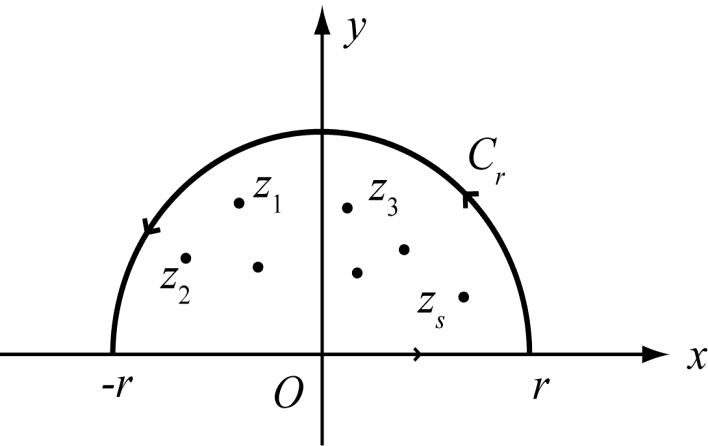
\includegraphics[keepaspectratio,alt={图5.3 上半圆周线及其中的极点}]{figures/05-留数理论及其应用/fig-p22-fe74c3b0.png}}
\caption{图5.3 上半圆周线及其中的极点}
\end{figure}

由留数定理，

\[
\int_{-r}^{r}R(x)\mathrm e^{\alpha\mathrm i x}\,\mathrm dx
+\int_{C_r}R(z)\mathrm e^{\alpha\mathrm i z}\,\mathrm dz
=2\pi\mathrm i\sum_{k=1}^{s}\operatorname{Res}\bigl[R(z)\mathrm e^{\alpha\mathrm i z},z_k\bigr].
\]

又 \(n-m\ge1\)，故当 \(|z|\) 充分大时，有

\[
|R(z)|\le\frac{M}{|z|}.
\]

因此

\[
\begin{aligned}
\Bigl|\int_{C_r}R(z)\mathrm e^{\alpha\mathrm i z}\,\mathrm dz\Bigr|
&=\Bigl|\int_{0}^{\pi}R(r\mathrm e^{\mathrm i\theta})\mathrm e^{\alpha\mathrm i r\mathrm e^{\mathrm i\theta}}\cdot \mathrm i r\mathrm e^{\mathrm i\theta}\,\mathrm d\theta\Bigr|\\
&\le M\int_{0}^{\pi}\mathrm e^{-\alpha r\sin\theta}\,\mathrm d\theta
=2M\int_{0}^{\pi/2}\mathrm e^{-\alpha r\sin\theta}\,\mathrm d\theta .
\end{aligned}
\]

当 \(0\le\theta\le\dfrac{\pi}{2}\)
时，\(\sin\theta\ge\dfrac{2\theta}{\pi}\)（Jordan 不等式），所以有

\[
\Bigl|\int_{C_r}R(z)\mathrm e^{\alpha\mathrm i z}\,\mathrm dz\Bigr|
\le2M\int_{0}^{\pi/2}\mathrm e^{-\alpha r\frac{2\theta}{\pi}}\,\mathrm d\theta
=\frac{M\pi}{\alpha r}\,\bigl(1-\mathrm e^{-\alpha r}\bigr)\to0\quad(r\to\infty).
\]

\begin{quote}
\textbf{注} 幻灯片此处写为
\(\dfrac{M\pi}{2r}(1-\mathrm e^{-\alpha r})\)，漏掉了分母中的
\(\alpha\)。按 Jordan 不等式严格计算应为
\(\dfrac{M\pi}{\alpha r}(1-\mathrm e^{-\alpha r})\)。
\end{quote}

当 \(r\to\infty\)
时，\(\displaystyle\int_{C_r}R(z)\mathrm e^{\alpha\mathrm i z}\,\mathrm dz\to0\)，得

\[
\boxed{\displaystyle\int_{-\infty}^{+\infty}R(x)\mathrm e^{\alpha\mathrm i x}\,\mathrm dx
=2\pi\mathrm i\sum_{k=1}^{s}\operatorname{Res}\bigl[R(z)\mathrm e^{\alpha\mathrm i z},z_k\bigr]} .
\]

分开实、虚部，即

\[
\int_{-\infty}^{+\infty}R(x)\cos\alpha x\,\mathrm dx
+\mathrm i\int_{-\infty}^{+\infty}R(x)\sin\alpha x\,\mathrm dx
=2\pi\mathrm i\sum_{k=1}^{s}\operatorname{Res}\bigl[R(z)\mathrm e^{\alpha\mathrm i z},z_k\bigr].
\]

\textbf{例 5.9} 求积分

\[
\int_{-\infty}^{+\infty}\frac{\cos x}{x^{2}+4x+5}\,\mathrm dx .
\]

\textbf{解} 设

\[
R(z)=\frac{1}{z^{2}+4z+5},
\]

则 \(R(z)\) 的分母高于分子二次，实轴上无奇点，上半平面只有一个一阶极点
\(z=-2+\mathrm i\)。于是

\[
\begin{aligned}
\int_{-\infty}^{+\infty}\frac{\mathrm e^{\mathrm i x}}{x^{2}+4x+5}\,\mathrm dx
&=2\pi\mathrm i\operatorname{Res}\bigl[R(z)\mathrm e^{\mathrm i z},-2+\mathrm i\bigr]\\
&=2\pi\mathrm i\lim_{z\to-2+\mathrm i}\bigl(z-(-2+\mathrm i)\bigr)R(z)\mathrm e^{\mathrm i z}\\
&=2\pi\mathrm i\lim_{z\to-2+\mathrm i}\frac{\mathrm e^{\mathrm i z}}{z+2+\mathrm i}
=2\pi\mathrm i\cdot\frac{\mathrm e^{-1-2\mathrm i}}{2\mathrm i}
=\pi\mathrm e^{-1-2\mathrm i},\\
\int_{-\infty}^{+\infty}\frac{\cos x}{x^{2}+4x+5}\,\mathrm dx
&=\operatorname{Re}\bigl[\pi\mathrm e^{-1-2\mathrm i}\bigr]
=\pi\mathrm e^{-1}\cos 2 .
\end{aligned}
\]

\subsection{\texorpdfstring{5.2.3 特殊定积分举例
I：\(\displaystyle\int_{0}^{+\infty}\frac{\sin x}{x}\,\mathrm dx\)}{5.2.3 特殊定积分举例 I：\textbackslash displaystyle\textbackslash int\_\{0\}\^{}\{+\textbackslash infty\}\textbackslash frac\{\textbackslash sin x\}\{x\}\textbackslash,\textbackslash mathrm dx}}\label{ux7279ux6b8aux5b9aux79efux5206ux4e3eux4f8b-idisplaystyleint_0inftyfracsin-xxmathrm-dx}

\textbf{例 5.10} 计算积分
\(\displaystyle\int_{0}^{+\infty}\frac{\sin x}{x}\,\mathrm dx\) 的值。

\textbf{解} 取函数

\[
f(z)=\frac{\mathrm e^{\mathrm i z}}{z},
\]

并取周线如图：上半平面大圆弧 \(C_R\)、小圆弧 \(C_r\)（绕过原点
\(z=0\)）及实轴上的两段之和。

\begin{figure}
\centering
\pandocbounded{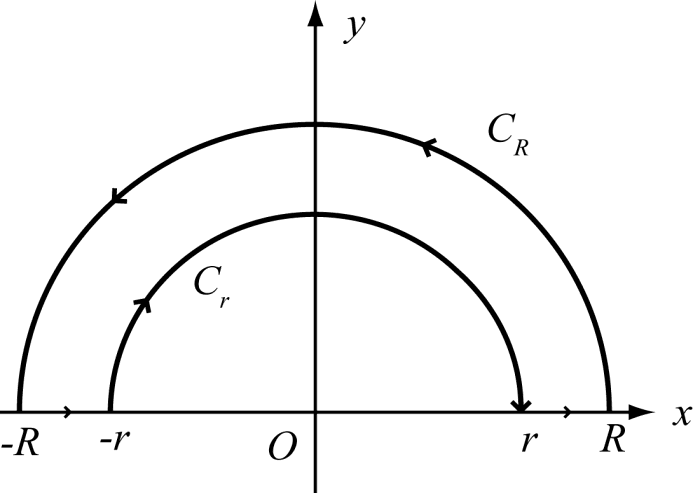
\includegraphics[keepaspectratio,alt={图5.4 避开原点的半圆周线}]{figures/05-留数理论及其应用/fig-p26-9e5100a0.png}}
\caption{图5.4 避开原点的半圆周线}
\end{figure}

在此周线中 \(f(z)\) 是解析的（\(z=0\)
已被小圆弧绕开），由柯西积分定理，得

\[
\int_{-R}^{-r}\frac{\mathrm e^{\mathrm i x}}{x}\,\mathrm dx
+\int_{C_r}\frac{\mathrm e^{\mathrm i z}}{z}\,\mathrm dz
+\int_{r}^{R}\frac{\mathrm e^{\mathrm i x}}{x}\,\mathrm dx
+\int_{C_R}\frac{\mathrm e^{\mathrm i z}}{z}\,\mathrm dz
=0 .
\]

令 \(x=-t\)，则有

\[
\int_{-R}^{-r}\frac{\mathrm e^{\mathrm i x}}{x}\,\mathrm dx
=-\int_{r}^{R}\frac{\mathrm e^{-\mathrm i t}}{t}\,\mathrm dt
=-\int_{r}^{R}\frac{\mathrm e^{-\mathrm i x}}{x}\,\mathrm dx .
\]

所以

\[
\int_{r}^{R}\frac{\mathrm e^{\mathrm i x}-\mathrm e^{-\mathrm i x}}{x}\,\mathrm dx
+\int_{C_R}\frac{\mathrm e^{\mathrm i z}}{z}\,\mathrm dz
+\int_{C_r}\frac{\mathrm e^{\mathrm i z}}{z}\,\mathrm dz
=0,
\]

即

\[
2\mathrm i\int_{r}^{R}\frac{\sin x}{x}\,\mathrm dx
+\int_{C_R}\frac{\mathrm e^{\mathrm i z}}{z}\,\mathrm dz
+\int_{C_r}\frac{\mathrm e^{\mathrm i z}}{z}\,\mathrm dz
=0 .
\]

由于

\[
\Bigl|\int_{C_R}\frac{\mathrm e^{\mathrm i z}}{z}\,\mathrm dz\Bigr|
\le\int_{0}^{\pi}\frac{\bigl|\mathrm e^{\mathrm i R\mathrm e^{\mathrm i\theta}}\bigr|}{R}\cdot R\,\mathrm d\theta
=\int_{0}^{\pi}\mathrm e^{-R\sin\theta}\,\mathrm d\theta
=2\int_{0}^{\pi/2}\mathrm e^{-R\sin\theta}\,\mathrm d\theta
\le\frac{\pi}{R}\bigl(1-\mathrm e^{-R}\bigr),
\]

故

\[
\lim_{R\to\infty}\int_{C_R}\frac{\mathrm e^{\mathrm i z}}{z}\,\mathrm dz=0 .
\]

又因为

\[
\frac{\mathrm e^{\mathrm i z}}{z}
=\frac{1}{z}+\mathrm i-\frac{z}{2!}+\cdots+\mathrm i^{n}\frac{z^{n-1}}{n!}+\cdots
=\frac{1}{z}+\varphi(z),
\]

其中 \(\varphi(z)\) 在 \(z=0\) 处解析，且
\(\varphi(0)=\mathrm i\)。因此当 \(|z|\) 充分小时，可设
\(|\varphi(z)|\le2\)。由于

\[
\int_{C_r}\frac{\mathrm e^{\mathrm i z}}{z}\,\mathrm dz
=\int_{C_r}\frac{\mathrm dz}{z}+\int_{C_r}\varphi(z)\,\mathrm dz,
\]

而

\[
\int_{C_r}\frac{\mathrm dz}{z}
=\int_{\pi}^{0}\frac{\mathrm i r\mathrm e^{\mathrm i\theta}}{r\mathrm e^{\mathrm i\theta}}\,\mathrm d\theta
=-\mathrm i\pi,
\qquad
\Bigl|\int_{C_r}\varphi(z)\,\mathrm dz\Bigr|\le2\pi r\to0,
\]

故有

\[
\lim_{r\to0}\int_{C_r}\frac{\mathrm e^{\mathrm i z}}{z}\,\mathrm dz=-\pi\mathrm i .
\]

令 \(R\to\infty\)，\(r\to0\)，则有

\[
2\mathrm i\int_{0}^{+\infty}\frac{\sin x}{x}\,\mathrm dx-\pi\mathrm i=0,
\]

即

\[
\boxed{\displaystyle\int_{0}^{+\infty}\frac{\sin x}{x}\,\mathrm dx=\frac{\pi}{2}} .
\]

\subsection{\texorpdfstring{5.2.4 形如
\(\displaystyle\int_{0}^{2\pi}R(\sin\theta,\cos\theta)\,\mathrm d\theta\)
的积分}{5.2.4 形如 \textbackslash displaystyle\textbackslash int\_\{0\}\^{}\{2\textbackslash pi\}R(\textbackslash sin\textbackslash theta,\textbackslash cos\textbackslash theta)\textbackslash,\textbackslash mathrm d\textbackslash theta 的积分}}\label{ux5f62ux5982-displaystyleint_02pirsinthetacosthetamathrm-dtheta-ux7684ux79efux5206}

设 \(R(x,y)\) 是两个变量 \(x,y\) 的有理函数。令
\(z=\mathrm e^{\mathrm i\theta}\)，那么

\[
\sin\theta=\frac{1}{2\mathrm i}\bigl(\mathrm e^{\mathrm i\theta}-\mathrm e^{-\mathrm i\theta}\bigr)
=\frac{1}{2\mathrm i}\Bigl(z-\frac{1}{z}\Bigr)
=\frac{z^{2}-1}{2\mathrm i z},
\]

\[
\cos\theta=\frac{1}{2}\bigl(\mathrm e^{\mathrm i\theta}+\mathrm e^{-\mathrm i\theta}\bigr)
=\frac{1}{2}\Bigl(z+\frac{1}{z}\Bigr)
=\frac{z^{2}+1}{2z},
\]

\[
\mathrm d\theta=\frac{\mathrm dz}{\mathrm i z}.
\]

从而原积分化为沿正向单位圆周的积分：

\[
\int_{0}^{2\pi}R(\cos\theta,\sin\theta)\,\mathrm d\theta
=\oint_{|z|=1}R\left(\frac{z^{2}+1}{2z},\frac{z^{2}-1}{2\mathrm i z}\right)\frac{\mathrm dz}{\mathrm i z}
=\oint_{|z|=1}f(z)\,\mathrm dz,
\]

其中 \(f(z)\) 为 \(z\) 的有理函数，且在单位圆周 \(|z|=1\) 上分母不为零。

\textbf{例 5.11} 计算积分

\[
\int_{0}^{2\pi}\cos^{4}4\theta\,\mathrm d\theta .
\]

\textbf{解} 令
\(z=\mathrm e^{\mathrm i\theta}\ (0\le\theta\le2\pi)\)，则

\[
\cos4\theta=\frac{z^{4}+z^{-4}}{2}=\frac{z^{8}+1}{2z^{4}},
\]

所以

\[
\begin{aligned}
\int_{0}^{2\pi}\cos^{4}4\theta\,\mathrm d\theta
&=\oint_{|z|=1}\left(\frac{z^{4}+z^{-4}}{2}\right)^{4}\frac{\mathrm dz}{\mathrm i z}
=\frac{1}{\mathrm i}\oint_{|z|=1}\frac{(z^{8}+1)^{4}}{16z^{17}}\,\mathrm dz .
\end{aligned}
\]

在 \(0<|z|<1\) 内，被积函数的洛朗展开式为

\[
\frac{(z^{8}+1)^{4}}{16z^{17}}
=\frac{1}{16}z^{-17}+\frac{1}{4}z^{-9}+\frac{3}{8}z^{-1}+\cdots.
\]

所以
\(operatorname{Res}\Bigl[\dfrac{(z^{8}+1)^{4}}{16z^{17}},0\Bigr]=\dfrac38\)，从而

\[
\int_{0}^{2\pi}\cos^{4}4\theta\,\mathrm d\theta
=\frac{1}{\mathrm i}\left\{2\pi\mathrm i\cdot\frac{3}{8}\right\}
=\frac{3}{4}\pi .
\]

\subsection{5.2.5 特殊定积分举例 II：Fresnel
积分}\label{ux7279ux6b8aux5b9aux79efux5206ux4e3eux4f8b-iifresnel-ux79efux5206}

由于留数是与闭曲线上的复积分相联系的，因此利用留数来计算定积分需要有两个主要的转化过程：

\begin{enumerate}
\def\labelenumi{\arabic{enumi}.}
\tightlist
\item
  将定积分的\textbf{被积函数}转化为复函数；
\item
  将定积分的\textbf{积分区间}转化为复积分的闭路曲线。
\end{enumerate}

下面用此方法计算积分

\[
\int_{0}^{\infty}\cos x^{2}\,\mathrm dx,\qquad
\int_{0}^{\infty}\sin x^{2}\,\mathrm dx .
\]

应取函数
\(f(z)=\mathrm e^{\mathrm i z^{2}}\)，取积分周线如图（扇形周线：\(OA\)
为实轴上 \(0\le x\le r\)，\(AB\) 为以原点为圆心、半径 \(r\)、辐角从
\(0\) 到 \(\pi/4\) 的圆弧，\(BO\) 为辐角 \(\pi/4\) 的径向线段）。

\begin{figure}
\centering
\pandocbounded{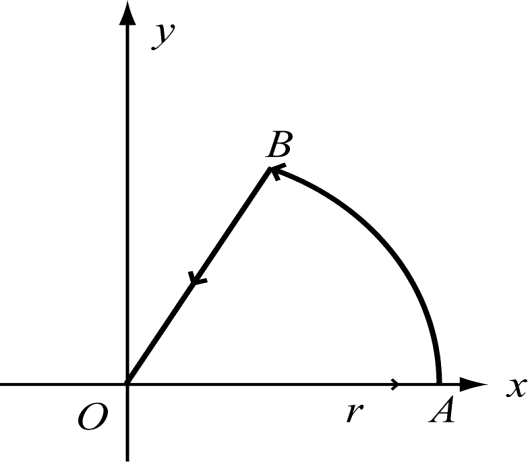
\includegraphics[keepaspectratio,alt={图5.5 计算 Fresnel 积分的扇形周线}]{figures/05-留数理论及其应用/fig-p31-29254dd8.png}}
\caption{图5.5 计算 Fresnel 积分的扇形周线}
\end{figure}

因为 \(f(z)\) 在闭周线内解析，由柯西积分定理，有

\[
\int_{OA}\mathrm e^{\mathrm i z^{2}}\,\mathrm dz
+\int_{AB}\mathrm e^{\mathrm i z^{2}}\,\mathrm dz
+\int_{BO}\mathrm e^{\mathrm i z^{2}}\,\mathrm dz
=0 .
\]

（1）当 \(z\) 在 \(OA\) 上时，\(z=x,\ 0\le x\le r\)，

\[
\int_{OA}\mathrm e^{\mathrm i z^{2}}\,\mathrm dz=\int_{0}^{r}\mathrm e^{\mathrm i x^{2}}\,\mathrm dx .
\]

（2）当 \(z\) 在 \(AB\)
上时，\(z=r\mathrm e^{\mathrm i\theta},\ 0\le\theta\le\dfrac{\pi}{4}\)，此时
\(\sin2\theta\ge\dfrac{4}{\pi}\theta\)，所以

\[
\bigl|\mathrm e^{\mathrm i z^{2}}\bigr|=\mathrm e^{-r^{2}\sin2\theta}\le\mathrm e^{-\frac{4}{\pi}r^{2}\theta},
\]

\[
\Bigl|\int_{AB}\mathrm e^{\mathrm i z^{2}}\,\mathrm dz\Bigr|
\le\int_{0}^{\pi/4}\mathrm e^{-\frac{4}{\pi}r^{2}\theta}\cdot r\,\mathrm d\theta
=\frac{\pi}{4r}\bigl(1-\mathrm e^{-r^{2}}\bigr)\to0\quad(r\to\infty).
\]

（3）当 \(z\) 在 \(BO\)
上时，\(z=x\mathrm e^{\mathrm i\pi/4},\ 0\le x\le r\)，则

\[
\int_{BO}\mathrm e^{\mathrm i z^{2}}\,\mathrm dz
=\int_{r}^{0}\mathrm e^{\mathrm i x^{2}\mathrm e^{\mathrm i\pi/2}}\cdot\mathrm e^{\mathrm i\pi/4}\,\mathrm dx
=-\mathrm e^{\mathrm i\pi/4}\int_{0}^{r}\mathrm e^{-x^{2}}\,\mathrm dx .
\]

令 \(r\to\infty\)，得

\[
\int_{0}^{\infty}\mathrm e^{\mathrm i x^{2}}\,\mathrm dx
+0-\mathrm e^{\mathrm i\pi/4}\int_{0}^{\infty}\mathrm e^{-x^{2}}\,\mathrm dx=0 .
\]

又

\[
\int_{0}^{\infty}\mathrm e^{-x^{2}}\,\mathrm dx=\frac{\sqrt\pi}{2},
\]

因此

\[
\int_{0}^{\infty}\mathrm e^{\mathrm i x^{2}}\,\mathrm dx
=\mathrm e^{\mathrm i\pi/4}\int_{0}^{\infty}\mathrm e^{-x^{2}}\,\mathrm dx
=\mathrm e^{\mathrm i\pi/4}\cdot\frac{\sqrt\pi}{2}.
\]

上式两边分别取实部和虚部，即得

\[
\boxed{\displaystyle\int_{0}^{\infty}\cos x^{2}\,\mathrm dx
=\int_{0}^{\infty}\sin x^{2}\,\mathrm dx
=\frac{1}{2}\sqrt{\frac{\pi}{2}}
=\frac{\sqrt{2\pi}}{4}} .
\]

\begin{quote}
\textbf{注} 幻灯片最后一行为
\(\dfrac12\cdot\dfrac{\sqrt\pi}{2}=\dfrac{\sqrt\pi}{4}\)，这是笔误。正确的应为
\(\dfrac12\sqrt{\dfrac{\pi}{2}}=\dfrac{\sqrt{2\pi}}{4}\)。
\end{quote}

\subsection{常见错误与注意点}\label{ux5e38ux89c1ux9519ux8befux4e0eux6ce8ux610fux70b9-13}

\begin{enumerate}
\def\labelenumi{\arabic{enumi}.}
\tightlist
\item
  \textbf{用 \(\int R(x)\mathrm dx\) 公式前必须验证
  \(n-m\ge2\)}。若只差一次，圆弧积分不一定为 \(0\)，此时要用含
  \(\mathrm e^{\alpha\mathrm i x}\) 的公式（\(n-m\ge1\)）。
\item
  \textbf{只取上半平面的极点}。留数求和只对 \(C_r\)
  内部的极点进行；实轴上的极点需另作处理（一般用小圆弧绕过）。
\item
  \textbf{Jordan 不等式}：当 \(0\le\theta\le\pi/2\) 时
  \(\sin\theta\ge\dfrac{2\theta}{\pi}\)。估算
  \(\displaystyle\int_0^{\pi/2}\mathrm e^{-\alpha r\sin\theta}\mathrm d\theta\)
  时，结果应为
  \(\dfrac{M\pi}{\alpha r}(1-\mathrm e^{-\alpha r})\)；幻灯片写成了
  \(\dfrac{M\pi}{2r}(1-\mathrm e^{-\alpha r})\)，漏掉了 \(\alpha\)。
\item
  \textbf{含 \(\mathrm e^{\alpha\mathrm i x}\)
  的积分常分开实、虚部求值}。例如例 5.9
  中，\(\int\cos x/(x^2+4x+5)\mathrm dx=\operatorname{Re}[\pi\mathrm e^{-1-2\mathrm i}]=\pi\mathrm e^{-1}\cos2\)，不要忘记取实部。
\item
  \textbf{例 5.8
  的乘子``\(2\pi\mathrm i\)''不要写成``\(2\pi\)''}。幻灯片写
  \(2\pi\left(\cdots\right)\) 是漏了 \(\mathrm i\)；严格应为
  \(2\pi\mathrm i\sum\operatorname{Res}\)。另外，幻灯片把这两个留数写成
  \(\dfrac{1+\mathrm i}{4\sqrt2\,\mathrm i}\) 与
  \(\dfrac{1-\mathrm i}{4\sqrt2\,\mathrm i}\)，等价于
  \(\dfrac{1-\mathrm i}{4\sqrt2}\) 与
  \(-\dfrac{1+\mathrm i}{4\sqrt2}\)。
\item
  \textbf{\(\sin x/x\) 的周线要避开原点}。因为 \(z=0\)
  是被积函数的可去奇点，周线必须用小圆弧绕开，且小圆弧积分
  \(\to-\pi\mathrm i\)。\(\lim_{r\to0}\int_{C_r}\mathrm e^{\mathrm i z}/z\,\mathrm dz=-\pi\mathrm i\)
  的符号很关键。
\item
  \textbf{Fresnel
  积分结果}：\(\int_0^\infty\cos x^2\mathrm dx=\int_0^\infty\sin x^2\mathrm dx=\dfrac12\sqrt{\dfrac{\pi}{2}}=\dfrac{\sqrt{2\pi}}{4}\)。不要把幻灯片中的
  \(\dfrac{\sqrt\pi}{4}\) 当成正确结果。
\end{enumerate}

\subsection{本节小结}\label{ux672cux8282ux5c0fux7ed3-13}

\begin{itemize}
\tightlist
\item
  \textbf{无理函数无穷积分}
  \(\int_{-\infty}^{\infty}R(x)\mathrm dx\)（\(n-m\ge2\)，\(Q\)
  无实零点）：取上半平面半圆，\(R\) 在圆弧上为
  \(O(|z|^{-2})\)，故圆弧积分趋于 \(0\)，结果是
  \(2\pi\mathrm i\sum\operatorname{Res}[R,z_k]\)（\(z_k\) 在上半平面）。
\item
  \textbf{含 \(\mathrm e^{\alpha\mathrm i x}\)
  的积分}（\(\alpha>0\)，\(n-m\ge1\)）：用 Jordan 不等式估计圆弧，结果
  \(2\pi\mathrm i\sum\operatorname{Res}[R\mathrm e^{\alpha\mathrm i z},z_k]\)；\(\alpha i\)
  的实部为负保证上半圆弧被``压''到 \(0\)。
\item
  \textbf{三角有理式周期积分}
  \(\int_0^{2\pi}R(\sin\theta,\cos\theta)\mathrm d\theta\)：令
  \(z=\mathrm e^{\mathrm i\theta}\)，化为单位圆周上的复积分
  \(\oint_{|z|=1}f(z)\mathrm dz\)。
\item
  \textbf{特殊定积分}：\(\int_0^\infty\frac{\sin x}{x}\mathrm dx=\frac{\pi}{2}\)；\(\int_0^\infty\cos x^2\mathrm dx=\int_0^\infty\sin x^2\mathrm dx=\frac{\sqrt{2\pi}}{4}\)。
\item
  核心思想：\textbf{用留数定理计算实定积分时，关键是``选对周线、让非待求部分趋于零、把待求部分与留数联系起来''}。
\end{itemize}

\newpage
